% 									Closing - Vorlage für Elektrotechnik
%                 					        2023 HTL Weiz
%----------------------------------------------------------------------------------------------------


%****************************************************************************************************
%========================================== A N H A N G =============================================
%****************************************************************************************************
%\newpage
%\addsec{Anhang}

%
\includepdf[pages=-]{./02_Documents/01_Sick-WL9-2P330S14.pdf}
%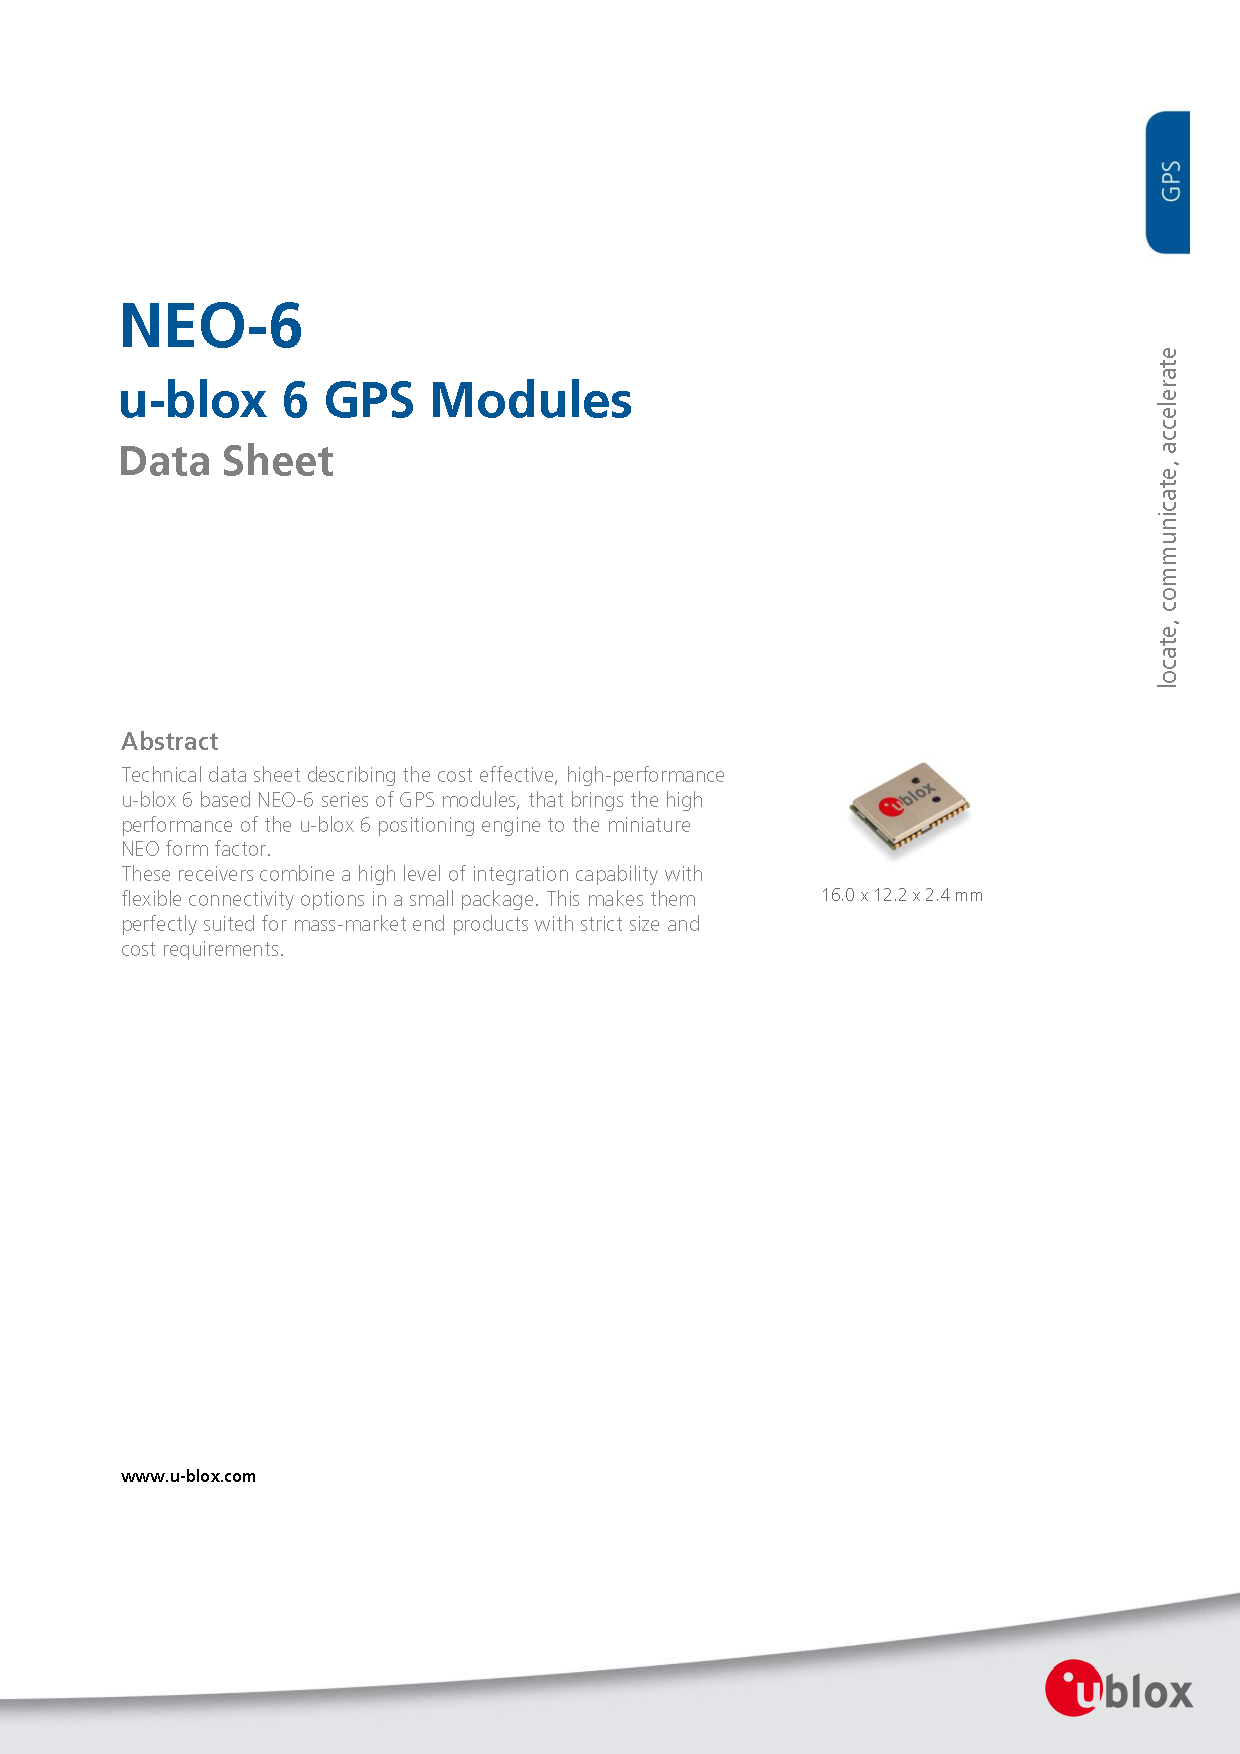
\includepdf[pages=-]{./02_Documents/02_UBlox-Neo-6MV2.pdf}
%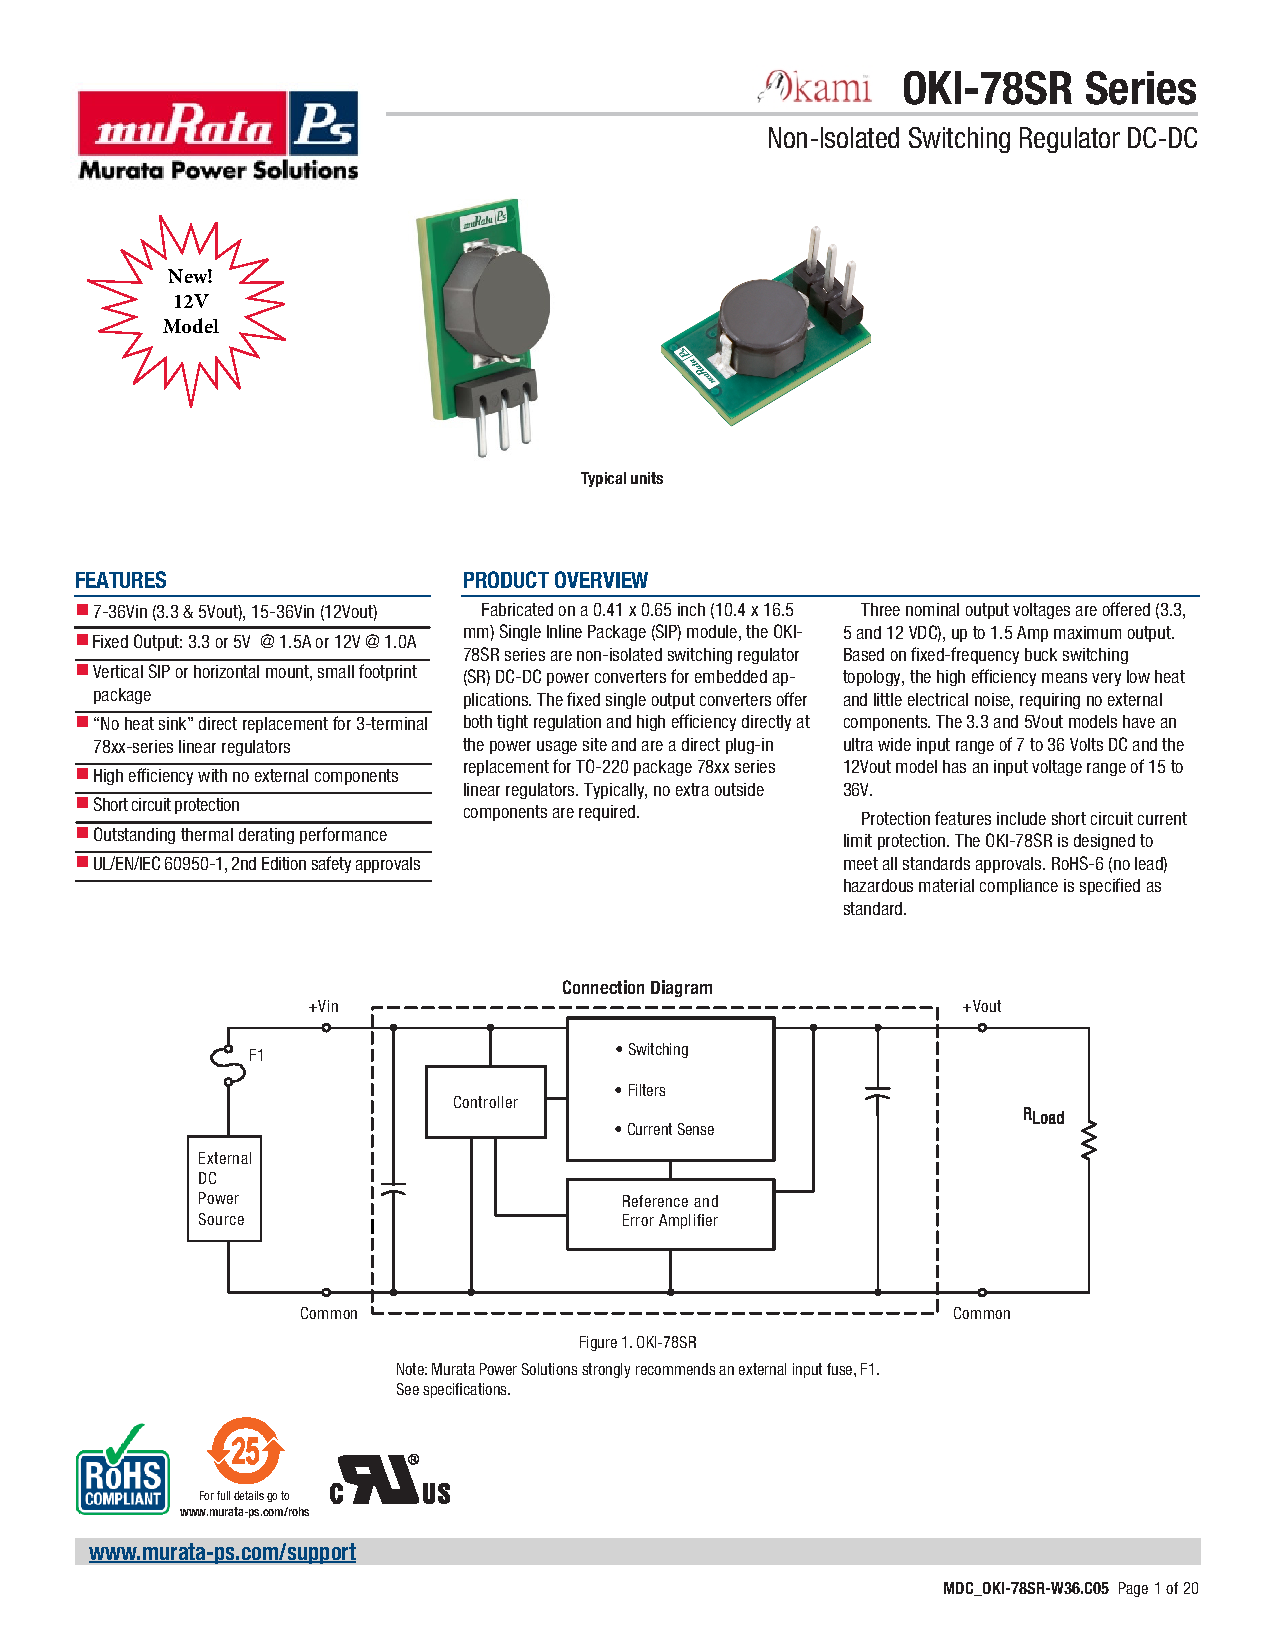
\includepdf[pages=-]{./02_Documents/03_Switching_Regulator.pdf}

%****************************************************************************************************
%============================ A B B I L D U N G S V E R Z E I C H N I S==============================
%****************************************************************************************************
\newpage
\listoffigures

%****************************************************************************************************
%============================= A B K Ü R Z U N G S V E R Z E I C H N I S ============================
%****************************************************************************************************
\newpage
\addsec{Abkürzungsverzeichnis}

\begin{acronym}[DBMS]	% Eckige Klammer: längste Abkürzung eintragen (Spalten werden angeglichen)
	\acro{DB}{Datenbank}
	\acro{GUI}{Graphical User Interface}
	\acro{DBMS}{Datenbank-Management-System}
	\acro{RasPi}{Raspberry Pi}
	\acro{DHCP}{Dynamic Host Configuration Protocol}
	\acro{µC}{Mikrocontroller}
	\acro{RTC}{Real Time Clock}
\end{acronym}


\newpage

%============================== L I T E R A T U R V E R Z E I C H N I S =============================

\printbibliography

\newpage

